\section{Detailed Design AODCS and pointing}
\label{sec:DDaodcs}
This section will describe the detailed design of the \ac{AODCS} and the pointing mechanism. The subsystem and also this section is split up in a number of parts. Section \ref{subsec:ADS} will treat the attitude determination, section \ref{subsec:ACS} deals with the attitude control, section \ref{subsec:ODS} is describes orbit determination, section \ref{subsec:OCS} discusses the orbit control and finally section \ref{subsec:point} describes the pointing mechanism. Section \ref{subsec:adcssum} gives a summery of the costs, weights and power usages of the components of the \ac{ADCS} and pointing mechanism.

%%%%%%%%%%%%%%%%%%%%%%%%%%%%%%%%%%%%%%%%%%%%%%%%%%%%%%%%%%%%%%%%%%%%%%%%%%%%%%%%%%%
\subsection{Attitude Determination}
\label{subsec:ADS}
In the Midterm Report \cite{midterm} sun sensors and a star tracker are chosen for the attitude determination of the satellites. Figure \ref{fig:sunstar} on page \pageref{fig:sunstar} shows the chosen options.

Eventually the chose for the sun sensors fell on the \ac{CoSS} from TNO \cite{tnoweb}. The mass of the instrument is 24 grams and it has a volume of 30 x 30 x 14.5 $mm^3$. It has a full cone view angle of 160${}^o$ and an accuracy of about 3 arcsec. The cost of one of these sun sensors is 11000 EUR, including all documentation. Since the sensors are passive no external power is needed. To cover the entire sphere around the satellite at least four of these sensors are needed. One placed at the top of the satellite, the others need to be on the sides of the satellites 60${}^o$ apart, i.e. one on a side panel and two at the corners of the plate opposite of that. It has to be noted for the processing of the data that analogue sun sensors in \ac{LEO} are sensitive to the influence of Earth albedo.

There are currently few star trackers available for micro-satellites. Aeroastro has developed one with a mass of the instrument is 375 grams and dimensions of 60 x 76.2 x 76.2 $mm^3$ (excluding the baffle). The instrument has a field of view of 24 x 30 degrees. It uses less than 2 Watts (1 Watt nominal). The attitude determination accuracy is about 90 arcsec. Up to 9 stars can be tracked at a time. ISIS \cite{cubesatshop} is working on a similar star tracker. Their dimensions are 50 x 50 x 100 $mm^3$. The instrument is planned to be ready for flight mid 2011 and will cost about 75000 EUR.

\begin{figure} [h]
\centering
\begin{tabular}{c c}
%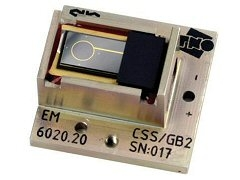
\includegraphics[width = 0.4\textwidth]{chapters/img/CoSS.jpg} & 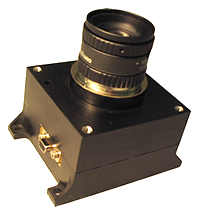
\includegraphics[width = 0.4\textwidth]{chapters/img/MSTracker.png}
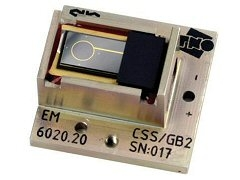
\includegraphics[width = 0.4\textwidth, bb=0 0 240px 180px]{chapters/img/CoSS.jpg} & 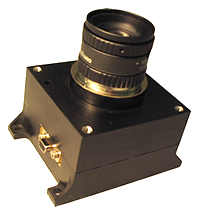
\includegraphics[width = 0.4\textwidth, bb=0 0 219px 215px]{chapters/img/MSTracker.png}
\end{tabular}
\caption[Sun sensor and star tracker]{The TNO Cosine Sun Sensor \cite{tnoweb} and the Aeroastro Miniature Star Tracker \cite{aeromst}}
\label{fig:sunstar}
\end{figure}

%%%%%%%%%%%%%%%%%%%%%%%%%%%%%%%%%%%%%%%%%%%%%%%%%%%%%%%%%%%%%%%%%%%%%%%%%%%%%%%%%%%

\subsection{Attitude Control}
\label{subsec:ACS}
The attitude control of the satellites is done by reaction wheels for manoeuvring and magneto torquers for desaturation (spinning down) of the wheels. Figure \ref{fig:catacs} on page \pageref{fig:catacs} shows a possible layout.

\begin{figure} [h]
\centering
%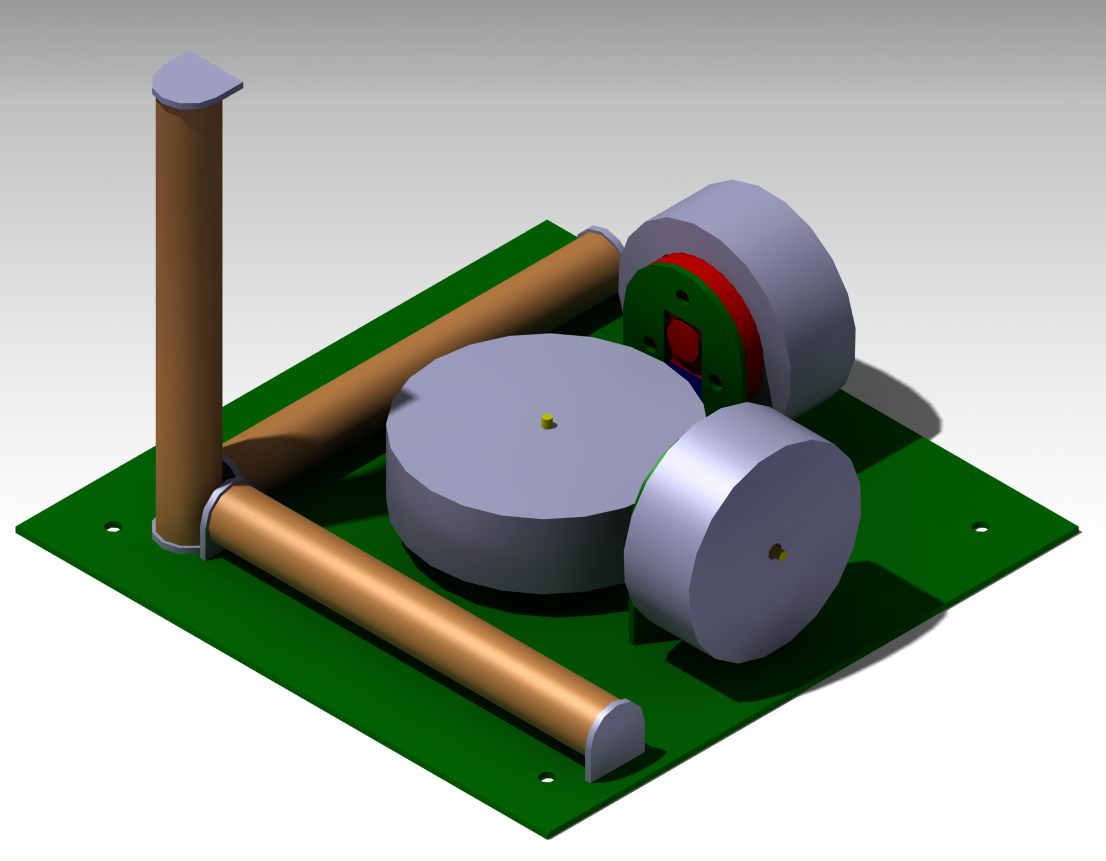
\includegraphics[width=0.8\textwidth]{chapters/img/AC_setup.png}
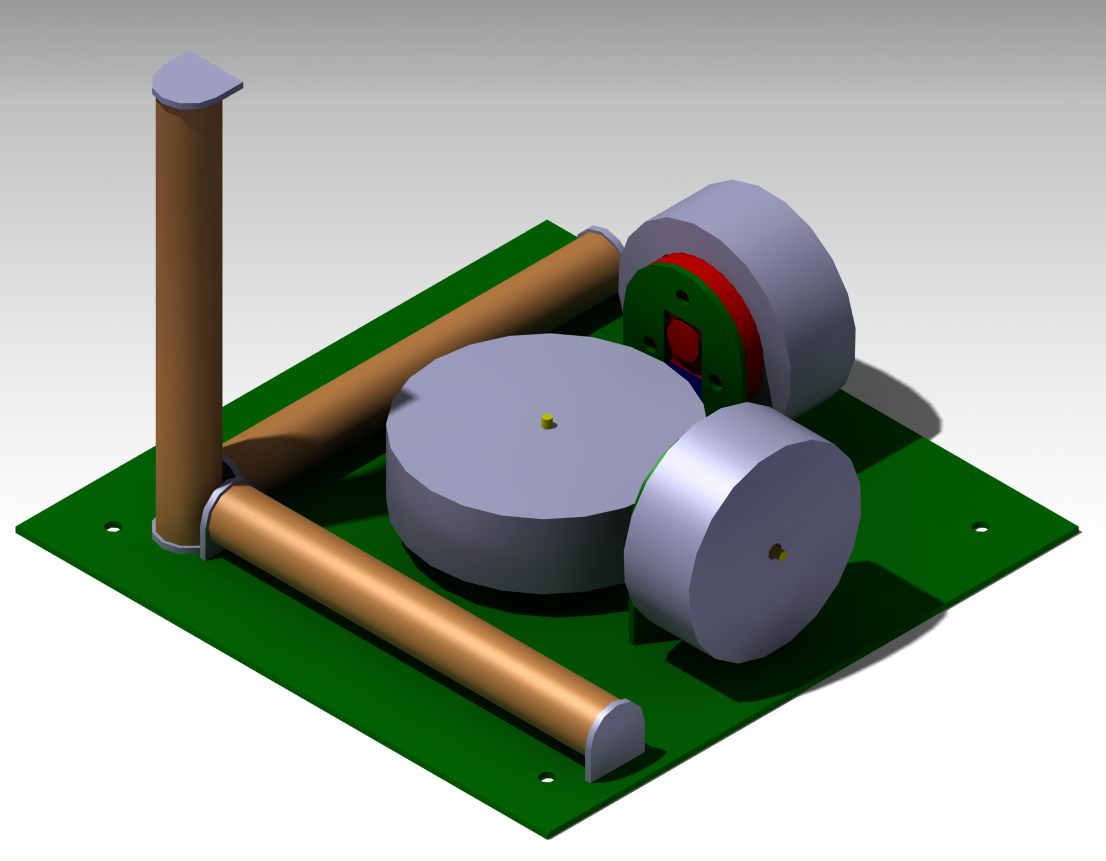
\includegraphics[width=0.8\textwidth, bb=0 0 1106px 861px]{chapters/img/AC_setup.png}
\caption[General layout of the attitude control subsystem]{General layout of the attitude control subsystem with reaction wheels and magneto torquers on all three axis.}
\label{fig:catacs}
\end{figure}

The sizing of the reaction wheels is done in such a way that the system is able to counter all disturbance torques that work on the satellite. The main disturbance torques are caused by the Earth's gravity gradient $T_g$(equation \ref{distgg}), Solar radiation $T_{sp}$ (equation \ref{distsr}), the Earth magnetic field $T_m$ (equation \ref{distmf}) and aerodynamics $T_a$ (equation \ref{distae}) \cite{larson}.

\begin{eqnarray}
T_g \,&=& \frac{3\mu}{2R^3} \left|I_z - I_y \right| \sin{2\theta} \label{distgg} \\
T_{sp} &=& \frac{F_s}{c}A_s\left(1+q\right)\cos{i}\left(c_{ps}-cg\right) \label{distsr} \\
T_m \,&=& DB \label{distmf} \label{distmf} \\
T_a \,&=& \dfrac{1}{2}\rho C_dAV^2 \left(c_{pa} -cg\right) \label{distae}
\end{eqnarray}
where $\mu$ is the Earth's gravitational constant 398600.4418 $km^3/s^2$, $R$ is the radius of the orbit, $I$ is the satellite inertia tensor, $\theta$ is the deviation from nadir, $F_s$ is the Solar constant 1367 $W/m^2$, $c$ is the speed of light 299792458 $m/s$, $q$ is the reflectance factor (0-1, typically 0.6), $i$ is the angle of incidence of the Sun, $c_{ps}$ is the center of solar pressure, $cg$ is the center of gravity, $D$ is the residual dipole of the satellite in $A\cdot m^2$, $B$ can be approximated as $2M/R^3$ in Tesla, where $M$ is the magnetic moment of the Earth 7.96 $T\cdot 10^{15} m^3$, $\rho$ is the local density in $kg/m^3$, $C_d$ is the drag coefficient of the satellite, $A$ is the surface area in $m^2$, $V$ is the satellite velocity and $c_{pa}$ is the center of aerodynamic pressure.

In the Master thesis of Angel Garza \cite{wheelmotor} he calculates the magnitude for a typical cubesat is in the order of $6\cdot 10^{-5}$ Nm. To have a good margin of safety the satellite needs to be able to produce at least twice that value. The torque a reaction wheel can produce is determined by

\begin{equation}
T_w = I_w \dot{\omega}_w
\label{wheeltorque}
\end{equation}

where $I_w$ is the inertia tensor of the wheel and $\dot{\omega}_w$ the angular acceleration. The inertia of the wheel depends on the dimensions.  The basic build-up of the wheels is a disk with a skirt around the motor giving the mass at a distance from the rotation axis as shown in figure \ref{fig:wheel} on page \pageref{fig:wheel}. The thickness $b$ of the skirt is 8 mm for the yaw wheel and 5 mm for the other two, since the yaw wheel is also used for the instrument pointing increasing the torque requirements. When the height of the wheel $h$ is chosen to be 1 $cm$ the small wheels have an inertia of $2.35\cot 10^{-6}\,kg\cdot m^2$, weighing 14.4 grams and the large wheel has an inertia of $5.13 \cot 10^{-6}\,kg\cdot m^2$ and weighs 24.7 grams.

\begin{figure}
\centering
%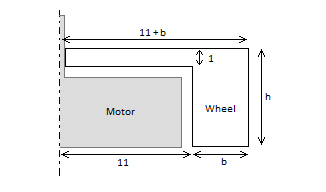
\includegraphics[width=0.3\textwidth]{chapters/img/reactionwheel.png}
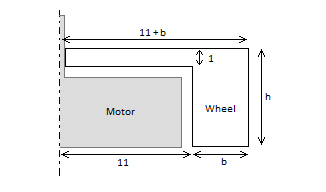
\includegraphics[width=0.3\textwidth, bb=0 0 216px 190px]{chapters/img/reactionwheel.png}
\caption[Basic reaction wheel]{The general layout of a one of the reaction wheels. The motor is depicted in grey, the wheel in white.}
\label{fig:wheel}
\end{figure}

The motors chosen for the reaction wheels are the Faulhauber 2209 Brushless DC-micromotors. The mass of the motor is 8.5 grams, the dimensions 22 x 22 x 17,5 $mm^3$ and the maximal rotation speed is 10000 rpm \cite{faulhaber}. They cost 176 EUR a piece. The maximum angular acceleration $\dot{\omega}_{max}$ they can perform is $1.03\cdot 10^3\,rad/s^2$, leading to a maximum torque of 2.42 and 5.28 mNm for the small and big wheels respectively. Although this is far more than required, the maximal angular acceleration will never be used because the wheels would saturate in about one second. 

The magneto torquers chosen are CubeSat Magnetorquers, which are available off the shelf from the cubesat webshop \cite{cubesatshop}. The weight is 30 grams and the diameter is 9 mm and the length is 70 mm. They can provide a torque of 0.2 $Am^2$. Three are required for the 3 axis desaturation. Price is 1150 EUR a piece. Three are needed to desaturate all three wheels.

%%%%%%%%%%%%%%%%%%%%%%%%%%%%%%%%%%%%%%%%%%%%%%%%%%%%%%%%%%%%%%%%%%%%%%%%%%%%%%%%%%%

\subsection{Orbit Determination}
\label{subsec:ODS}
The orbit determination and the time keeping is done by the navigation subsystem and is discussed in section \ref{}. %section where navigation can be found

%%%%%%%%%%%%%%%%%%%%%%%%%%%%%%%%%%%%%%%%%%%%%%%%%%%%%%%%%%%%%%%%%%%%%%%%%%%%%%%%%%%

\subsection{Orbit Control}
\label{subsec:OCS}
Before the constellation can even start making measurements the satellites need to go to their correct orbits and when they are in orbit they need to stay there for at least five years. In the midterm report it is derived that a thruster is required to keep the satellites in orbit for the entire mission lifetime. 

After launch all satellites will be in the same orbit. To get starboard and larboard satellites to their correct orbit at $\pm 2.18^o$ right ascension node a $\Delta V$ of 
\begin{equation}
\end{equation}
is required. For station keeping, ah well, can't say anything right now ...
I'll wait for Alex before writing the rest of this story. 

%%%%%%%%%%%%%%%%%%%%%%%%%%%%%%%%%%%%%%%%%%%%%%%%%%%%%%%%%%%%%%%%%%%%%%%%%%%%%%%%%%%

\subsection{Pointing Mechanism}
\label{subsec:point}
The pointing mechanism is use for pointing the receiver off-nadir towards the ground target. The right ascension difference of $2.18^o$ translates into a pointing difference of about $30^o$ in both directions. To be able to still make measurements when the distance between the satellites gets bigger a total design pointing angle of $80^o$ is chosen. The pointing of the instrument is done by a tumbler, drive by a wheel, connected to a harmonic gear box, attached to a stepper motor. The general layout can be seen in figure \ref{fig:point} on page \pageref{fig:point}. The different parts of the pointing mechanism will be discussed in reverse order in this section.

\begin{figure} [h]
\centering
%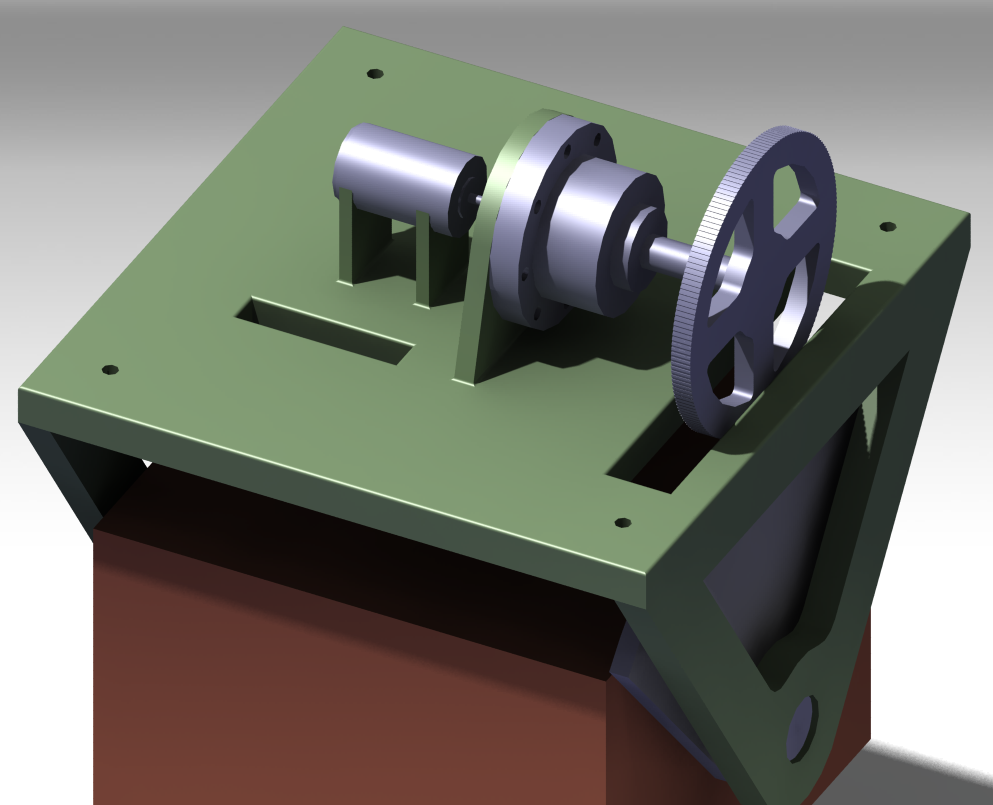
\includegraphics[width=0.8\textwidth]{chapters/img/point_setup.png}
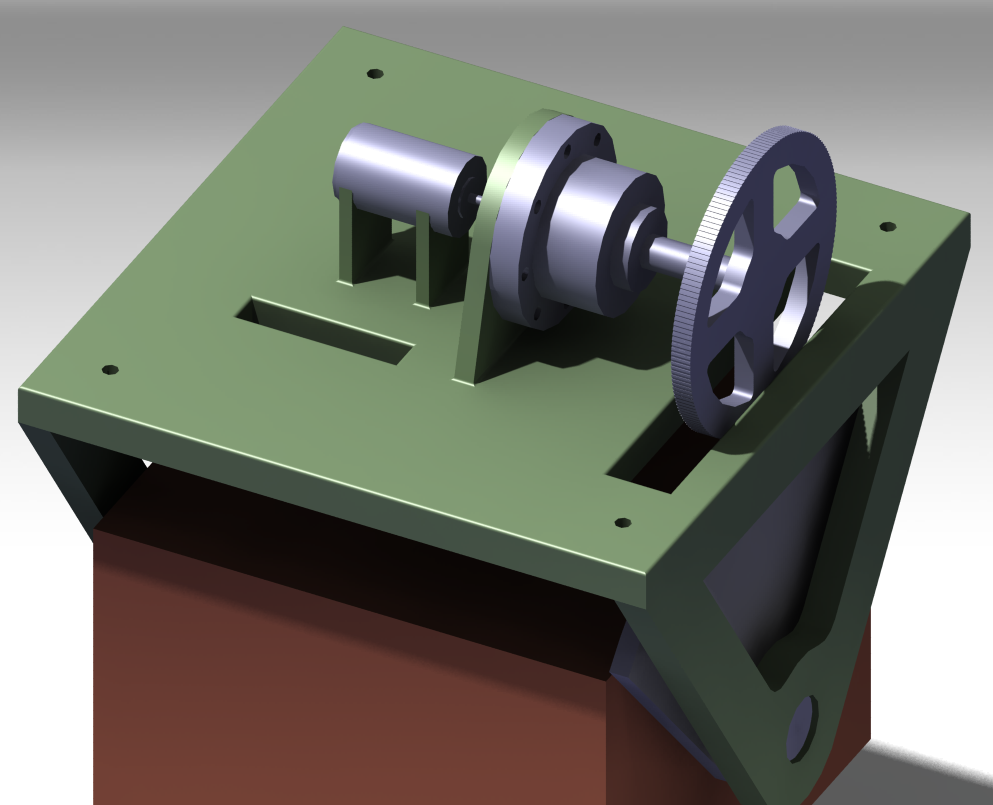
\includegraphics[width=0.8\textwidth, bb=0 0 895px 756px]{chapters/img/point_setup.png}
\caption[General layout of the receiver pointing mechanism]{General layout of the receiver pointing mechanism, with the stepper motor, harmonic drive and the tumbler.}
\label{fig:point}
\end{figure}

The selected stepper motor is a Faulhaber ADM1220. The nominal power is 0.6 Watts. The diameter of the motor is 12 mm, the length of the motor and the axis is 17.4 mm and the motor has a mass of 9 grams. The motor is capable of making 20 discrete steps, giving it a step angle of $18^o$. Naturally this is not accurate enough, so a gearbox is needed.

For the gearbox a harmonic drive is chosen \cite{harmonicdrive}. It is chosen because it has half the size, one third of the weight of a conventional gear. A Harmonic Drive CSF-8-50 is selected \cite{harmweb}. The gearbox has a gear ratio of 50:1, a diameter of 30 mm, a length of 22.1 mm and a mass of 26 g. With this set-up it is possible to make 20 x 50 = 1000 steps for a full circular rotation of the output axis. Divided over the $80^o$ of the possible pointing options this gives a pointing capability with steps of $0.08^o$.

The output of the harmonic drive is put into a wheel with the same circumference as the $80^o$ sweep of the tumbler, so a complete rotation of the wheel sweeps the receiver from one maximum to the other. This translates into a wheel with a radius of 22.15 mm and a tumbler with a radius of 59.85 mm from the rotation axis of the receiver. The pointing of the receiver can be read by an array of sensors reading a 10-bit ($2^10 = 1024$ steps) grey code from the side of the tumbler.

%%%%%%%%%%%%%%%%%%%%%%%%%%%%%%%%%%%%%%%%%%%%%%%%%%%%%%%%%%%%%%%%%%%%%%%%%%%%
\subsection{Summery}
\label{subsec:adcssum}
Table \ref{tab:adcspointbudget} on page \ref{tab:adcspointbudget} gives an overview of the costs, mass and power use of the different components of the \ac{ADCS} and the pointing mechanism for one satellite.
\begin{table}[h]
\begin{tabular}{l | c | c c | c c | c }
Subsystem component    & Number & Mass & Cost & Total mass & Total cost & Power (max)\\ 
                       &   & [g] & [EUR]& [g]  &[EUR] & [W]         \\ \hline \hline
Sun sensors            & 4 & 24  & 11000& 96   & 44000&  0 (0)      \\
Star trackers          & 1 & 375 & 75000& 375  & 75000&  1 (2)      \\ \hline
Reaction wheel motors  & 3 & 8.5 & 176  & 25.5 & 528  &  0.15 (1.5) \\
Reaction wheel disk    & 3 & 18  & 10*  & 54   & 30*  &  0 (0)      \\
Magneto torquers       & 3 & 30  & 1150 & 90   & 3450 &  1 (3)      \\ \hline
Stepper motor          & 1 & 9   & 112  & 9    & 112  &  0.6 (1.2)  \\
Harmonic drive         & 1 & 26  & 180* & 26   & 180* &  0 (0)      \\ 
Tumbler                & 1 & 22  & 10*  & 22   & 10*  &  0 (0)      \\ \hline
Total & & &                             & 814  & 123310& 2.75 (4.1 rms)
\end{tabular}
\caption[Mass and cost budget ADCS and pointing]{Mass and cost budget of different parts of the ADCS and pointing mechanism. Starred prices are estimations based on material and machining cost.}
\label{tab:adcspointbudget}
\end{table}